\documentclass[11pt]{article}
\usepackage[a4paper,margin=1in]{geometry}
\usepackage{amsmath,amssymb,amsthm,mathtools}
\usepackage{booktabs}
\usepackage{enumitem}
\usepackage{graphicx}
\usepackage{hyperref}
\usepackage[nameinlink,capitalise]{cleveref}
\usepackage[numbers,sort&compress]{natbib}

\newtheorem{theorem}{Theorem}[section]
\newtheorem{proposition}[theorem]{Proposition}
\newtheorem{corollary}[theorem]{Corollary}
\theoremstyle{remark}
\newtheorem{remark}[theorem]{Remark}
\newcommand{\norm}[1]{\left\lVert#1\right\rVert}
\newcommand{\C}{\mathbb C}
\newcommand{\cH}{\mathcal H}

\title{Moving-Cloud Renormalization and the Relative Determinant Gate\\
\large Why Fixed Double-Pole Cancellation Cannot Cross the Small-Noise Circle}
\author{Liang Wang}
\date{July 2026}

\begin{document}
\maketitle

\begin{abstract}
The intrinsic two-step program has reached trace-norm square transfer and
Fredholm determinants on shrinking disks, but its generic absolute
continuity estimate is nonuniform on fixed disks.  Independently, the
deterministic coefficient germ has the exact double pole
\[
 \widehat F_0(w)=\frac{H(w)}{(1-w/\lambda)^2},
 \qquad \lambda=1.678573510428322\ldots .
\]
This paper decides which pole renormalization can plausibly cross that circle.

For the exact finite cloud
$C_N(w)=\Pi_N(w/\lambda)^2$, the apparently natural fixed cancellation has
the identity
\[
 (1-w/\lambda)^2C_N(w)
 =\bigl(1-(w/\lambda)^{N+1}\bigr)^2.
\]
It converges uniformly to one on every strict interior disk, but diverges at
every fixed point $|w|>\lambda$.  Thus multiplication by the limiting scalar
pole factor is not a fixed-disk renormalization, even in the canonical model.

The positive replacement is an exact moving-cloud quotient.  If a finite-rank
reducing projection isolates the noisy cloud of $T_\sigma=B_\sigma^2$, then
the Fredholm determinant factors exactly as $D_\sigma=C_\sigma R_\sigma$.
A uniform trace-norm bound on the complementary block makes the residual
determinants a normal family on every fixed disk; trace-norm convergence gives
an explicit locally uniform determinant bound.  A coefficient deconvolution
lemma identifies any such limit with the deterministic numerator $H$.

A 256-bit Arb audit replays the archived RH-15 cloud coordinates.  At
$\sigma=10^{-4}$ the selected degree is seven, the centered two-step radius is
$1.8751435740$, and the observed zero-radius band is
$[1.7449450709,1.9816784182]$.  The recentered five-point edge profile has mean
error at most $0.03633$ and maximum error at most $0.11590$.  This supports the
moving factor geometrically but does not construct its Riesz projection or
bound the complement.  Stage A5 remains open with a sharper, operator-level
gate; no Hilbert--Polya or Riemann-hypothesis conclusion is made.
\end{abstract}

\noindent\textbf{Keywords:} Fredholm determinant; spectral cloud; pole
renormalization; trace ideal; normal family; small noise.

\medskip
\noindent\textbf{MSC 2020:} 47B10; 47B35; 47A55; 30D45; 65G20.

\section{The fixed-disk fork}

RH-46 proved that the deterministic symmetric two-step germ has a genuine
double pole at $w=\lambda$ and that the unrenormalized positive-noise entire
determinants cannot form a normal family on a disk crossing that point
\citep{WangDoublePole2026}.  RH-79 subsequently transferred conditional
intrinsic operator control to trace-norm squares and shrinking-disk
determinants, while exposing the generic fixed-disk factor
$\exp(O(R/\sigma))$ \citep{WangDiagonalTransfer2026}.

There are therefore two superficially similar operations:
\begin{enumerate}[leftmargin=2em]
 \item multiply by the fixed deterministic factor $(1-w/\lambda)^2$;
 \item divide by the finite spectral polynomial carried by the actual noisy
 cloud.
\end{enumerate}
The first operation cancels the limiting meromorphic pole germ.  The second
removes the finite-dimensional mechanism that resolves that pole at positive
noise.  The distinction is decisive on a disk crossing $|w|=\lambda$.

\section{Exact failure of fixed scalar cancellation}

Set
\[
 \Pi_N(q)=1+q+\cdots+q^N,
 \qquad C_N(w)=\Pi_N(w/\lambda)^2.
\]
This is the exact squared geometric cloud factor from RH-46.

\begin{theorem}[Fixed-pole cancellation dichotomy]
\label{thm:fixed-failure}
For $q=w/\lambda$,
\begin{equation}
 (1-q)^2C_N(w)=(1-q^{N+1})^2.
 \label{eq:exact-cancellation}
\end{equation}
Consequently, for every $0\le r<1$,
\begin{equation}
 \sup_{|q|\le r}
 \left|(1-q)^2C_N(\lambda q)-1\right|
 \le 2r^{N+1}+r^{2N+2}.
 \label{eq:interior-bound}
\end{equation}
At every fixed $q_0$ with $|q_0|>1$,
\begin{equation}
 \left|(1-q_0)^2C_N(\lambda q_0)\right|
 \ge \bigl(|q_0|^{N+1}-1\bigr)^2\longrightarrow\infty.
 \label{eq:exterior-growth}
\end{equation}
Hence the fixed-cancelled canonical family is not locally bounded on any disk
$|w|<R$ with $R>\lambda$.
\end{theorem}

\begin{proof}
The geometric identity $(1-q)\Pi_N(q)=1-q^{N+1}$ gives
\eqref{eq:exact-cancellation}.  Subtracting one and applying the triangle
inequality proves \eqref{eq:interior-bound}.  The reverse triangle inequality
gives \eqref{eq:exterior-growth}.  Every disk with $R>\lambda$ contains a real
point $q_0\in(1,R/\lambda)$, so pointwise unboundedness rules out local
boundedness.
\end{proof}

The theorem is stronger than a failure of one estimate: the fixed factor
fails in the exact model that generated the double pole.  At degree $N=64$,
the certified interior error is at most $1.01\times10^{-6}$ on $|q|\le0.8$,
while at the nearby exterior point $q=1.05$ the fixed-cancelled magnitude is
at least $5.2166\times10^2$.  The circle, not arithmetic precision, separates
the two regimes.

\section{The exact moving-cloud quotient}

Let $T_\sigma\in\mathcal S_1(\cH_\sigma)$ denote a two-step trace-class
operator.  A bounded finite-rank projection $P_\sigma$ is called a reducing
cloud projection when $P_\sigma T_\sigma=T_\sigma P_\sigma$.  Put
$Q_\sigma=I-P_\sigma$ and use the invariant direct sum
$\cH_\sigma=\operatorname{ran}P_\sigma\oplus\operatorname{ran}Q_\sigma$.

\begin{theorem}[Moving-cloud relative determinant]
\label{thm:relative}
For every reducing cloud projection,
\begin{equation}
 D_\sigma(w):=\det(I-wT_\sigma)
 =C_\sigma(w)R_\sigma(w),
 \label{eq:block-factor}
\end{equation}
where
\[
 C_\sigma(w)=\det_{\operatorname{ran}P_\sigma}
  (I-wT_\sigma|_{\operatorname{ran}P_\sigma}),
 \qquad
 R_\sigma(w)=\det_{\operatorname{ran}Q_\sigma}
  (I-wT_\sigma|_{\operatorname{ran}Q_\sigma}).
\]
Both factors are entire and the quotient $D_\sigma/C_\sigma$ extends through
all cloud zeros as the entire function $R_\sigma$.

If the residual blocks, transported to a common Hilbert space, satisfy
\begin{equation}
 \sup_\sigma\norm{S_\sigma}_1\le K,
 \label{eq:uniform-complement}
\end{equation}
then for every $R>0$,
\begin{equation}
 \sup_{|w|\le R}|R_\sigma(w)|\le e^{RK}.
 \label{eq:normal-bound}
\end{equation}
Thus the residual family is normal on $\C$.  If additionally
$\norm{S_\sigma-S_0}_1\le\varepsilon_\sigma\to0$, then
\begin{equation}
 \sup_{|w|\le R}|R_\sigma(w)-R_0(w)|
 \le R\varepsilon_\sigma
 e^{1+R\norm{S_\sigma}_1+R\norm{S_0}_1}.
 \label{eq:relative-continuity}
\end{equation}
\end{theorem}

\begin{proof}
Commutation makes $T_\sigma$ block diagonal on the invariant direct sum, and
the Fredholm determinant is multiplicative across trace-class direct sums.
The standard inequalities
$|\det(I+A)|\le e^{\norm A_1}$ and
\[
 |\det(I+A)-\det(I+B)|
 \le\norm{A-B}_1e^{1+\norm A_1+\norm B_1}
\]
give \eqref{eq:normal-bound} and \eqref{eq:relative-continuity}
\citep{Simon2005}.
\end{proof}

The full trace norm of $T_\sigma=B_\sigma^2$ may grow like
$\sigma^{-1}$, which caused the RH-79 absolute determinant barrier.  The
criterion \eqref{eq:uniform-complement} asks whether that growth is confined
to the extracted finite cloud.  If so, the exponential contains $RK$ rather
than $O(R/\sigma)$.

\section{Identification of the residual limit}

Normality alone gives subsequences.  The coefficient bridge identifies their
only possible limit.

\begin{proposition}[Coefficient deconvolution]
\label{prop:deconvolution}
Let $D_j=C_jR_j$ be germs at zero with $C_j(0)=1$.  Suppose the Taylor
coefficients of $D_j$ and $C_j$ converge coefficientwise to those of
$D_0=C_0R_0$, where $C_0(0)=1$.  Then every Taylor coefficient of $R_j$
converges to the corresponding coefficient of $R_0$.

If the $R_j$ are locally bounded on a connected domain containing zero, then
$R_j\to R_0$ locally uniformly there whenever $R_0$ has a holomorphic
continuation to that domain.
\end{proposition}

\begin{proof}
Writing $d_{j,m}=\sum_{k=0}^m c_{j,k}r_{j,m-k}$ and using $c_{j,0}=1$
determines $r_{j,m}$ recursively from lower coefficients.  Induction proves
coefficient convergence.  Local boundedness gives subsequential compactness
by Montel's theorem; every subsequential limit has the same derivatives at
zero and therefore equals $R_0$ by the identity theorem \citep{Conway1978}.
Uniqueness upgrades subsequential convergence to full convergence.
\end{proof}

For the ideal cloud, the coefficients of $C_N$ converge to those of
$(1-w/\lambda)^{-2}$.  Together with the RH-46 coefficient bridge,
\cref{prop:deconvolution} identifies a normal relative limit with the
holomorphic numerator $H$.  For the actual noisy dynamics, however, one must
still prove both the cloud-factor coefficient bridge and
\eqref{eq:uniform-complement}.

\section{Validated replay of the archived cloud}

The numerical audit reads the decimal cloud coordinates archived by RH-15
\citep{WangBulkScattering2026}.  Arb at 256-bit precision propagates those
decimals through radial centering, the two-step cloud product, and the finite
geometric edge profile.  This validates the replay arithmetic, not the
upstream floating eigensolver.

\begin{table}[ht]
\centering
\small
\begin{tabular}{rrrrrr}
\toprule
$\sigma$ & $N$ & center & mismatch & zero-radius band & mean error\\
\midrule
$10^{-2}$ & 3 & 2.70658 & 0.61243 & [2.19694,3.61314] & 0.00855\\
$2\!\times\!10^{-3}$ & 4 & 2.00651 & 0.19537 & [1.84466,2.16455] & 0.01399\\
$5\!\times\!10^{-4}$ & 5 & 1.99166 & 0.18652 & [1.78723,2.25347] & 0.04079\\
$2\!\times\!10^{-4}$ & 6 & 1.90530 & 0.13507 & [1.75548,2.06217] & 0.03644\\
$10^{-4}$ & 7 & 1.87515 & 0.11711 & [1.74495,1.98168] & 0.03633\\
\bottomrule
\end{tabular}
\caption{Selected rows from the seven-level cloud audit.  Mismatch is relative
to $\lambda$; mean error is over $s=-1,-1/2,0,1/2,1$.  Bounds are rounded
outward from the archived Arb certificate.}
\label{tab:cloud}
\end{table}

The center moves substantially toward $\lambda$, and the finest recentered
profile remains close to the exact finite-section shape.  Yet degree seven is
far too small to infer asymptotic cloud identification, the center is still
$11.71\%$ high, and no complement determinant is contained in the archived
data.  The evidence selects the moving-factor route without closing it.

\begin{figure}[ht]
\centering
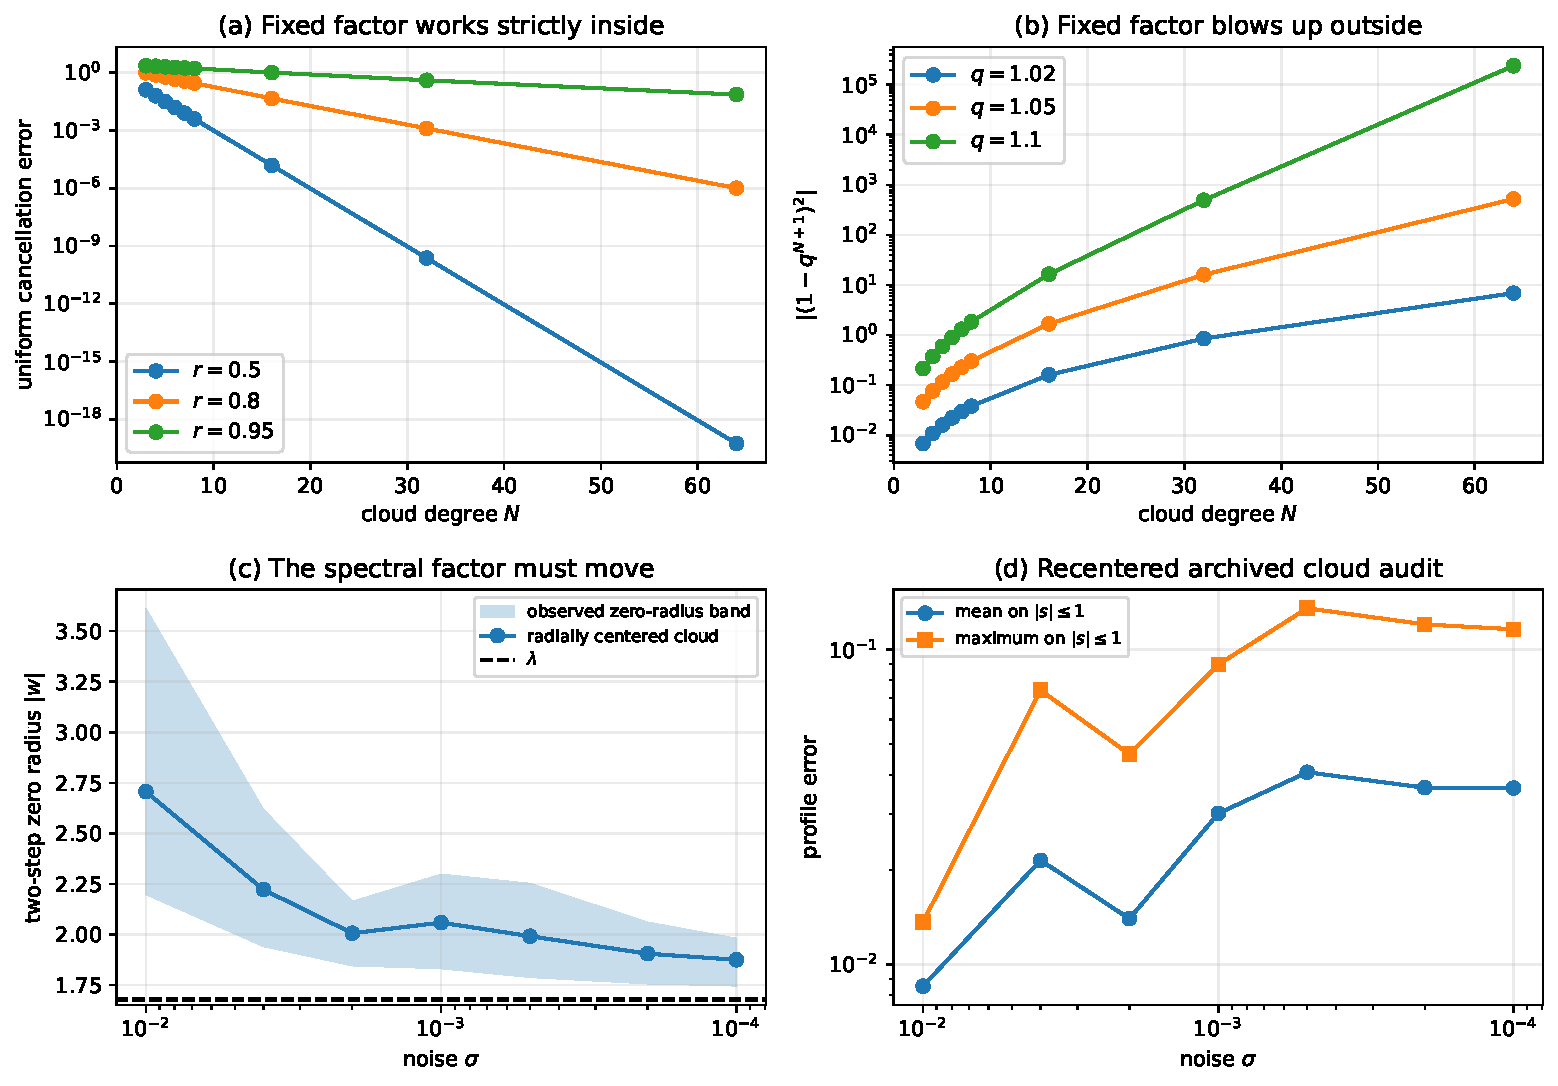
\includegraphics[width=\textwidth]{figures/moving_cloud_relative_determinant.pdf}
\caption{The RH-80 fork.  Fixed cancellation converges strictly inside the
pole circle (a) and grows outside it (b).  The archived noisy zero band moves
toward the deterministic pole (c), while recentered finite-section agreement
remains a floating-cloud diagnostic (d).}
\label{fig:route}
\end{figure}

\section{Route consequence and theorem boundary}

RH-80 eliminates a tempting but incorrect fixed-disk shortcut.  Multiplying
by $(1-w/\lambda)^2$ only recovers the deterministic numerator on strict
interior disks.  Crossing the pole circle requires division by the actual
finite spectral cloud, followed by a uniform theorem for its complementary
block.

The next strict gate is therefore:
\begin{enumerate}[leftmargin=2em]
 \item construct a moving Riesz projection whose finite determinant is the
 actual cloud polynomial;
 \item prove that the complementary two-step block is uniformly trace class,
 or prove a sharper relative determinant bound with the same normal-family
 consequence;
 \item establish the cloud coefficient bridge so that the residual limit is
 identified with $H$.
\end{enumerate}

The exact factorization and its sufficient convergence theorem are
unconditional functional analysis.  Their application to the present noisy
dynamical family is conditional on the three gates above.  Stage A5 is not
closed.  Nothing here constructs a self-adjoint Hilbert--Polya operator,
proves a $T\log T$ law or prime-power trace formula, identifies zeta zeros, or
proves the Riemann Hypothesis.

\bibliographystyle{plainnat}
\bibliography{references}

\end{document}

